\section{Verification through Sensor Data}
Verification is a broad topic in buildings that refers to verifying several things about building sensor metadata or through
the sensor data.  Both cases are related to physical states are relationships that are assumed by the user and are either
true and empirically observable or not.  If not, the end user or process should be informed and that inconsistencies should
be immediately addressed.  This is even more of an issues as building begin to reply more and more on software.

In this section we introduce some of the tools that we use for verification as discuss the 4 types of verification
that exists in buildings.  We also present an overview approach for 3 of them.

\subsection{Correlation}
Throughout this work, we make extensive use of the correlation coefficient function defined as: 

\begin{displaymath}
r(X,Y) = r_{X, Y} = \frac{\sum_{i=1}^{n} (X_{i} - \overline{X})(Y_{i} - \overline{Y})}
{\sqrt{\sum_{i=1}^{n} (X_{i} - \overline{X})^2}\sqrt{\sum_{i=1}^{n} (Y_{i} - \overline{Y})^2}}
\end{displaymath}

where $X$, $Y$ are separate sets of values, $n$ is the total number of sample points in 
each set, and $\overline{X}$ is the mean value of $X$ (same for $\overline{Y}$ and Y).  % over the entire sampling period.
For each pair of sensors, we compute the corrcoeff to ascertain the relationship between them.


\subsection{Empirical Mode Decomposition} \label{emd}
Another important tool that we used is empirical mode decomposition.  We use it partition the empiriical data is its constituent
sub-signals and examine what those sub-signals tell us about its behavior.  We also use it to examine how signal behavve between
one another at certain bands of importance that contain important physical information.

Empirical Mode Decomposition (EMD) \cite{huang:emd1998} is a technique that decomposes a signal and reveals intrinsic patterns, 
trends, and noise.
This technique has been widely applied to a variety of datasets, including climate variables~\cite{lee:climateEMD2011}, medical data~\cite{blanco:bioMed2008}, speech signals~\cite{huang:signalProc2006,hasan:ieeeletter2009}, and image processing~\cite{nunes:vision2005}.
% for example, it helped to uncover the global surface temperature trends\cite{}, solar activity patterns and predicts climate variables .
EMD's effectiveness relies on its empirical, adaptive and intuitive approach.
In fact, this technique is designed to efficiently decompose both non-stationary and non-linear signals without requiring any 
a priori basis functions or tuning.  

EMD decomposes a signal into a set of oscillatory components called intrinsic mode functions (IMFs). 
An IMF satisfies two conditions: (1) it contains the same number of extrema and zero crossings (or differ at most by one); (2) the two 
IMF envelopes defined by its local maxima and local minima are symmetric with respect to zero.  Consequently, 
 IMFs are functions that directly convey the amplitude and frequency modulations.

% EMD is an iterative sifting process that extracts IMFs step by step; each step seeks for the IMF with the highest frequency, then the computed IMF is removed from the data and the residual data are used as input for the next step.
EMD is an iterative algorithm that extracts IMFs step by step by using the so-called sifting process \cite{huang:emd1998}; each step seeks for the IMF with the highest frequency by sifting, then the computed IMF is removed from the data and the residual data are used as input for the 
next step.
The process stops when the residual data becomes a monotonic function from which no more IMF can be extracted.

We formally describe the EMD algorithm as follows: 
\begin{enumerate}
\item Sifting process: For a current signal $h_0=X$, let $m_0$ be the mean of its upper and lower envelopes as determined from a cubic-spline interpolation of local maxima and minima.
\item The estimated local mean $m_0$ is removed from the signal, giving a first component: $h_1 = h_0-m_0$
\item The sifting process is iterated, $h_1$ taking the place of $h_0$. Using its upper and lower envelopes, a new local mean $m_1$ is computed and $h_2 = h_1-m_1$.
\item The procedure is repeated $k$ times until $h_k=h_{k-1}-m_{k-1}$ is an IMF according to the two conditions above.
\item This first IMF is designated as $c_1 = h_k$, and contains the component with shortest periods. We extract it from the signal to produce a residual: $r_1 = X - c_1$.  Steps 1 to 4 are repeated on the residual signal $r_1$, providing IMFs $c_j$ and residuals $r_j  = r_{j-1}-c_j$, for $j$ from $1$ to $n$.
\item The process stops when residual $r_n$ contains no more than 3 extrema.
\end{enumerate}

The result of EMD is a set of IMFs $c_i$ and the final residue $r_n$, such as: \[X=\sum^{n}_{i=1}c_i+r_n\]
where the size of the resulting set of IMFs ($n$) depends on the original signal $X$ and $r_n$ represents the trend of 
the data (see \emph{IMFs} in Figure~\ref{fig:diagram1}).

For this work we implemented a variant of EMD called Complete Ensemble EMD~\cite{torres:icassp2012}.
This algorithm computes EMD several times with additional noise, it allows us to efficiently analyze signals that have 
flat sections (i.e. consuming no electricity in our case). % and permits us to solve the \emph{EMD mode mixing problem}.

\subsection{Reaggregation of Intrinsic Mode Functions} \label{methodo:corr}
By applying EMD to energy consumption signals we obtain a set of IMFs that precisely describe the devices consumption 
patterns at different frequency bands.  Therefore, we can focus our analysis on the smaller time scales, ignoring the dominant 
patterns that prevent us from effectively analyzing raw signals.

However, comparing the IMFs obtained from different signals is also not trivial,
 because EMD is empirically uncovering IMFs from the data there is no guarantee that the two IMFs $c_i^1$ and $c_i^2$ obtained from two distinct signals $S^1$ and $S^2$ represent data at the same frequency domain.
Directly comparing $c_i^1$ and $c_i^2$ is meaningless unless we confirm that they belong to the same frequency domain.

There are numerous techniques to retrieve IMF frequencies~\cite{huang:aada2009}.  
In this work we take advantage of the Generalized Zero Crossing (GZC)~\cite{huang:patent2006} because it is a simple and robust 
estimator of the instantaneous IMF frequency \cite{huang:aada2009}.
GZC is a direct estimation of IMF instantaneous frequency using critical points defined as the zero crossings and local extrema 
(round dots in Figure~\ref{fig:gzc}).
Formally, given a data point $p$, GZC measures the quarter ($T_4$), the two halves ($T_2^x$), and the four full periods ($T_1^y$), $p$   
belong to (see Figure~\ref{fig:gzc}) and the instantaneous period is computed as:
\[T=\frac{1}{7}\{4T_4+(2T_2^1+2T_2^2)+(T_1^1+T_1^2+T_1^3+T_1^4)\}\]

\begin{figure}
\begin{center}
 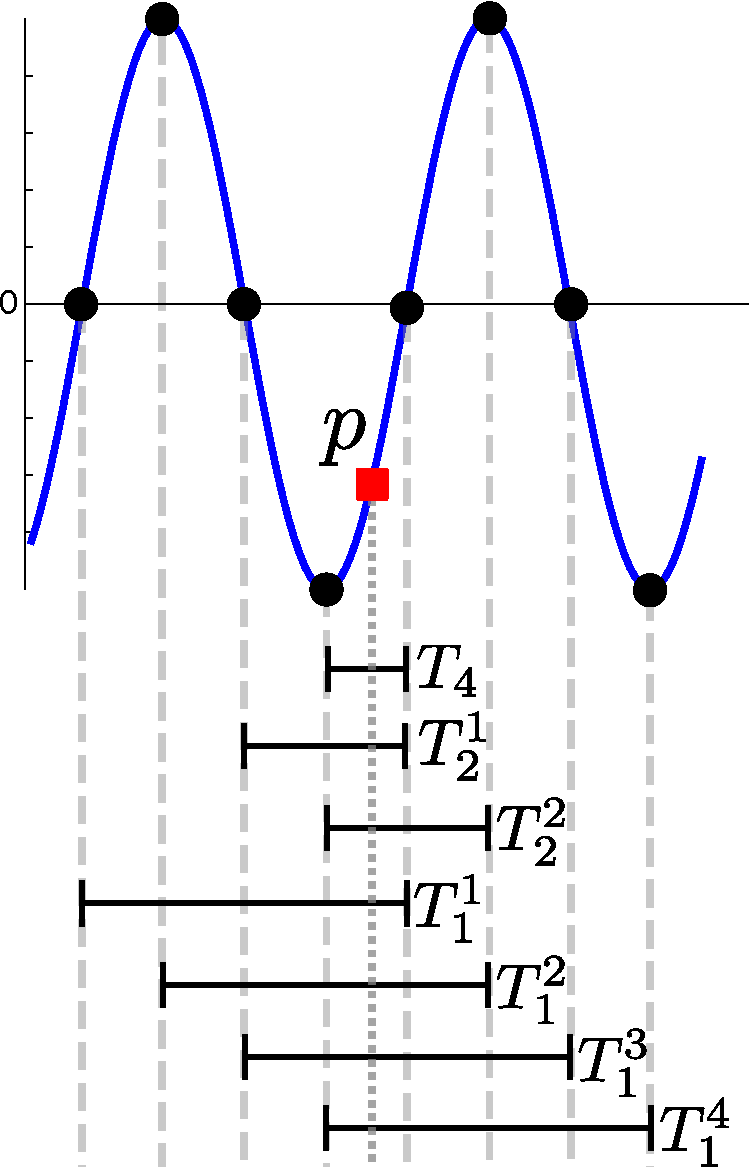
\includegraphics[width=.25\textwidth]{figs/gzc.pdf}
 \end{center}
 \caption{Generalized Zero Crossing: the local mean period at the point $p$ is computed from one quarter period $T_4$, two half periods $T_2^x$ and four full periods $T_1^y$ (where $x=1, 2$, and, $y=1,2,3,4$).}
 \label{fig:gzc}
\end{figure}

Since all points $p$ between two critical points have the same instantaneous period GZC is local down to a quarter period.
Hereafter, we refer to the time scale of an IMF as the average of the instantaneous periods along the whole IMF.
Because the time scale of each IMF depends on the original signal, we propose the following to efficiently compare IMFs from different signals.
We cluster IMFs with respect to their time scales and partially reconstruct each signal by aggregating its IMFs from the 
same cluster.  Then, we directly compare the partial signals of different devices.

EMD yields distinct components in different time scales and we compute the instantaneous frequencies \cite{IF} of IMFs using Generalized Zero-Crossing \cite{GZC}.  We break the time scales into four frequency bands:
\begin{itemize}
\item High Frequency: a time scale smaller than 30 minutes, mainly reflecting the operation characteristics of devices and noise in system. 
\item Medium Frequency: a time scale between 30 minutes and 6 hours, which is within the time span of daily activities inside a building.
\item Low Frequency: a time scale between 6 hours and 7 days. %This category usually captures patterns repeated in a longer cycle, say, days. 
\item Residue: everything has a time scale longer than 7 days and shows long-term patterns, such as seasonal changes.
\end{itemize}

Later in this thesis we will explain how we use the medium-frequency band for both spatial verification and functional verification.  We discuss
the 4 types of verification in the next section.





